\documentclass[handout]{beamer}
%\documentclass{beamer}
\usepackage{tikz}
\def\checkmark{\tikz\fill[scale=0.4](0,.35) -- (.25,0) -- (1,.7) -- (.25,.15) -- cycle;} 
\usepackage{pifont}
\newcommand{\xmark}{\ding{55}}
\usepackage{tikz}
\usepackage{biblatex}
\usetheme{PaloAlto}
\title{Hierarchical models, ODEs, and model selection}
\author[Ben Lambert]{Ben Lambert\inst{1}\\ \texttt{ben.lambert@stats.ox.ac.uk}}
\usepackage{datetime}
\date{}
\institute[University of Oxford]{
\inst{1}Department of Statistics\\
University of Oxford}
\beamertemplatenavigationsymbolsempty
\setbeamertemplate{sidebar left}{}
\usepackage{caption}
\captionsetup{font=footnotesize}
\usepackage[utf8]{inputenc}
\usepackage{amsmath}
\usepackage{multimedia}
\usepackage{animate}
\usepackage{graphics}
\usepackage{graphicx}
\usepackage[makeroom]{cancel}
\usepackage{relsize}
\usepackage{minted}

\makeatletter
\newcommand\mathcircled[1]{%
  \mathpalette\@mathcircled{#1}%
}
\newcommand\@mathcircled[2]{%
  \tikz[baseline=(math.base)] \node[draw,circle,inner sep=1pt] (math) {$\m@th#1#2$};%
}
\makeatother

\makeatletter
\def\maxwidth{ %
	\ifdim\Gin@nat@width>\linewidth
	\linewidth
	\else
	\Gin@nat@width
	\fi
}
\makeatother

\definecolor{fgcolor}{rgb}{0.345, 0.345, 0.345}
\newcommand{\hlnum}[1]{\textcolor[rgb]{0.686,0.059,0.569}{#1}}%
\newcommand{\hlstr}[1]{\textcolor[rgb]{0.192,0.494,0.8}{#1}}%
\newcommand{\hlcom}[1]{\textcolor[rgb]{0.678,0.584,0.686}{\textit{#1}}}%
\newcommand{\hlopt}[1]{\textcolor[rgb]{0,0,0}{#1}}%
\newcommand{\hlstd}[1]{\textcolor[rgb]{0.345,0.345,0.345}{#1}}%
\newcommand{\hlkwa}[1]{\textcolor[rgb]{0.161,0.373,0.58}{\textbf{#1}}}%
\newcommand{\hlkwb}[1]{\textcolor[rgb]{0.69,0.353,0.396}{#1}}%
\newcommand{\hlkwc}[1]{\textcolor[rgb]{0.333,0.667,0.333}{#1}}%
\newcommand{\hlkwd}[1]{\textcolor[rgb]{0.737,0.353,0.396}{\textbf{#1}}}%
\usepackage{xcolor}
\definecolor{orangeBright}{RGB}{243,146,0}
\definecolor{blueBright}{RGB}{54,169,225}
\definecolor{pinkBright}{RGB}{214,11,82}
\definecolor{shadecolor}{rgb}{.97, .97, .97}
\definecolor{messagecolor}{rgb}{0, 0, 0}
\definecolor{warningcolor}{rgb}{1, 0, 1}
\definecolor{errorcolor}{rgb}{1, 0, 0}

\usepackage{framed}
\makeatletter
\newenvironment{kframe}{%
	\def\at@end@of@kframe{}%
	\ifinner\ifhmode%
	\def\at@end@of@kframe{\end{minipage}}%
\begin{minipage}{\columnwidth}%
	\fi\fi%
	\def\FrameCommand##1{\hskip\@totalleftmargin \hskip-\fboxsep
		\colorbox{shadecolor}{##1}\hskip-\fboxsep
		% There is no \\@totalrightmargin, so:
		\hskip-\linewidth \hskip-\@totalleftmargin \hskip\columnwidth}%
	\MakeFramed {\advance\hsize-\width
		\@totalleftmargin\z@ \linewidth\hsize
		\@setminipage}}%
{\par\unskip\endMakeFramed%
	\at@end@of@kframe}
\makeatother

\definecolor{shadecolor}{rgb}{.97, .97, .97}
\definecolor{messagecolor}{rgb}{0, 0, 0}
\definecolor{warningcolor}{rgb}{1, 0, 1}
\definecolor{errorcolor}{rgb}{1, 0, 0}
\newenvironment{knitrout}{}{} % an empty environment to be redefined in TeX

\usepackage{alltt}
\IfFileExists{upquote.sty}{\usepackage{upquote}}{}

\bibliography{Bayes}

\begin{document}

\begin{frame}
\titlepage
\end{frame}

\begin{frame}
	\frametitle{Lecture outcomes}
	
	By the end of this lecture you should:
	\begin{enumerate}
		\item<2-> Understand what is meant by a hierarchical model.
		\item<3-> Appreciate some of the benefits of using hierarchical models.
		\item<4-> Know how to think Bayesianly about ordinary differential equation models (ODEs), and use Stan to code up simple examples.
		\item<5-> Understand how to think Bayesianly about model selection.
	\end{enumerate}
	
\end{frame}

\section{Thinking hierarchically}
\frame{\tableofcontents[currentsection]}
\begin{frame}
	\frametitle{Example: EU referendum}
	
	\begin{itemize}
		\item<2-> Imagine a dystopian future where the UK decides to hold a referendum on its membership of the EU.
		\item<3-> Have data from 20 polls on EU membership carried out over the past month (fake data).
		\item<4-> Polls conducted by a range of different agencies.
		\item<5-> The sample size of each poll is 10.
		\item<6-> Ultimately want to use model to forecast the result of the EU referendum.
	\end{itemize}
	
	\begin{figure}[ht]
		\centerline{\includegraphics[width=0.8\textwidth]{figures/brexit2.jpg}}
	\end{figure}
	
\end{frame}


\begin{frame}
	\frametitle{EU referendum: data}
	\begin{figure}[ht]
		\centerline{\includegraphics[width=1\textwidth]{figures/lec6_euFakeDataVis.pdf}}
	\end{figure}
\end{frame}

\begin{frame}
	\frametitle{EU referendum: complete pooling model}
	\onslide<2-> Suppose that the we assume that the data across all polls are:
	\begin{itemize}
		\item<3-> Independent.
		\item<4-> Identically distributed.
	\end{itemize}
	\onslide<5-> Sample size is fixed and data are discrete $\implies$ binomial likelihood:
	
	\onslide<6->
	\begin{equation}
	Pr(X=X_i|\theta ) = \theta^{X_i} (1-\theta)^{10-X_i}
	\end{equation}
	
	\onslide<7->
	where $X_i$ is the number of people voting 'remain' in poll $i$, and $\theta$ is the probability that a randomly-chosen person will vote `remain'.
	
	\onslide<8->
	\textbf{Important:} we are assuming that $\theta$ is the same across all polls.
	
\end{frame}

\begin{frame}[fragile]
	\frametitle{EU referendum: complete pooling model in Stan}
\begin{minted}{stan}
data {
  int<lower=1> K; // number of polls
  int<lower=0> X[K]; // numbers voting 'remain'
  int<lower=1> N; // sample size
}
parameters {
  real<lower=0,upper=1> theta;
} 
model {
  for (i in 1:K){
    X[i] ~ binomial(N,theta);
  }
}
\end{minted}
	\onslide<2-> Implicitly $\implies$ that we are using a uniform prior on (0,1) for theta.
\end{frame}

\begin{frame}[fragile]
	\frametitle{EU referendum: complete pooling model results}
	\begin{knitrout}\scriptsize
		\definecolor{shadecolor}{rgb}{0.969, 0.969, 0.969}\color{fgcolor}\begin{kframe}
			\begin{alltt}
				\hlkwd{print}\hlstd{(fit,}\hlkwc{probs} \hlstd{=} \hlkwd{c}\hlstd{(}\hlnum{0.25}\hlstd{,} \hlnum{0.5}\hlstd{,} \hlnum{0.75}\hlstd{))}
			\end{alltt}
			\begin{verbatim}
			## Inference for Stan model: lec6_euBinomialHomgeneousSimple.
			## 4 chains, each with iter=1000; warmup=500; thin=1; 
			## post-warmup draws per chain=500..
			## 
			##          mean se_mean   sd     25%     50%     75% n_eff Rhat
			## theta    0.57    0.00 0.03    0.55    0.57    0.59   656 1.01
			## lp__  -206.59    0.02 0.65 -206.75 -206.32 -206.17   774 1.00
			\end{verbatim}
		\end{kframe}
	\end{knitrout}
	
	\onslide<2->
	$\implies$ all looks ok.
\end{frame}

\begin{frame}
	\frametitle{EU referendum: complete pooling model results}
	\begin{figure}[ht]
		\centerline{\includegraphics[width=1\linewidth]{figures/lec6_euHomogeneousPosterior.pdf} }
	\end{figure}
\end{frame}


\begin{frame}
	\frametitle{ EU referendum: complete pooling model posterior predictive checks}
	Count number of times that 9 or more people vote 'remain', and find 4/30 cases.
	
	\begin{figure}[ht]
		\centerline{\includegraphics[width=0.95\textwidth]{figures/lec6_euReferendumHighlighted.pdf}}
	\end{figure}
	
\end{frame}

\begin{frame}
	\frametitle{ EU referendum: complete pooling model posterior predictive checks}
	Repeat for 2000 simulated data series; for each simulated dataset counting the number of $X_i\geq 9$.
	
	\begin{figure}[ht]
		\centerline{\includegraphics[width=0.85\textwidth]{figures/lec6_euHomoPPCRuns1.pdf}}
	\end{figure}
	
\end{frame}

\begin{frame}
	\frametitle{ EU referendum: complete pooling model posterior predictive checks}
	Low probability of replicating this aspect of real data.
	
	\begin{figure}[ht]
		\centerline{\includegraphics[width=0.85\textwidth]{figures/lec6_euHomoPPCRuns2.pdf}}
	\end{figure}
	
\end{frame}

\begin{frame}
	\frametitle{EU referendum: complete pooling model summary}
	\begin{itemize}
		\item<2-> Assumed a model where the probability of a polled individual intending to vote 'remain' is \textbf{identical} across all polls.
		\item<3-> However polls were conducted over a range of time by a range of agencies, each with their own methodology $\implies$ sampling method, exact interview process etc vary.
		\item<4-> Therefore assuming a common $\theta$ across polls is too strong an assumption.
		\item<5-> $\implies$ model will \textbf{understate} true uncertainty.
	\end{itemize}
	
	\onslide<6-> 
	$\implies$ try the opposite extreme where we allow a different $\theta_i$ for each poll.
	
\end{frame}

\begin{frame}
	\frametitle{EU referendum: heterogeneous model}
	\onslide<2-> For each poll $i$ we assume a binomial likelihood:
	
	\onslide<3->
	\begin{equation}
	Pr(X=X_i|\theta_i) = \theta_i^{X_i} (1-\theta_i)^{10-X_i}
	\end{equation}
	
	\onslide<4-> where $\theta_i$ is the probability of a interviewee indicating they intend to vote `remain' in the referendum.

    \vspace{0.5cm}
 
	\onslide<5-> By allowing $\theta_i$ to vary across polls $\implies$ \textbf{different} data generating processes for each poll.
	
\end{frame}

\begin{frame}[fragile]
	\frametitle{EU referendum: heterogeneous model}
	\begin{minted}{stan}
data {
  int<lower=1> K; // number of polls
  int<lower=0> X[K]; // numbers voting 'remain'
  int<lower=1> N; // sample size
}
parameters {
  real<lower=0,upper=1> theta[K]; // now array
} 
model {
  for (i in 1:K){ 
    X[i] ~ binomial(N,theta[i]);// select element
  }
}
	\end{minted}
	\onslide<2->
	$\implies$ only two changes to homogeneous model necessary.
\end{frame}

\begin{frame}
	\frametitle{Heterogeneous model results}
	\begin{figure}[ht]
		\centerline{\includegraphics[width=1\textwidth]{figures/lec6_euHeteroPosterior.pdf}}
	\end{figure}
	
	\onslide<2-> $\implies$ large uncertainty associated with each $\theta_i$.
	
\end{frame}

\begin{frame}
	\frametitle{Heterogeneous model posterior predictive checks}
	\onslide<2-> Compare again occurrence of 9+/10 'remain' voters with real data; where 4/30.
	
	\begin{figure}[ht]
		\centerline{\includegraphics[width=0.9\textwidth]{figures/lec6_euReferendumHighlighted.pdf}}
	\end{figure}
	
\end{frame}

\begin{frame}
	\frametitle{Heterogeneous model posterior predictive checks}
	For 2000 posterior predictive samples.
	
	\begin{figure}[ht]
		\centerline{\includegraphics[width=0.85\textwidth]{figures/lec6_euHeteroPPCHist1.pdf}}
	\end{figure}
	
\end{frame}

\begin{frame}
	\frametitle{Heterogeneous model posterior predictive checks}
	$\implies$ better than complete pooling model.
	
	\begin{figure}[ht]
		\centerline{\includegraphics[width=0.85\textwidth]{figures/lec6_euHeteroPPCHist2.pdf}}
	\end{figure}
	
\end{frame}

\begin{frame}
	\frametitle{Heterogeneous model problems}
	\begin{itemize}
		\item<2-> Heterogeneous model is a better fit to the data than fully-pooled $\impliedby$ is overfitting the data?
		\item<3-> However not clear what we should now forecast for the polls? Should we use:
		\begin{itemize}
			\item[-]<4-> Estimate from one poll.
			\item[-]<5-> Average across point estimates for all polls.
		\end{itemize}
		\item<6-> Further how should we quantify our uncertainty?
	\end{itemize}
	
\end{frame}

\begin{frame}
	\frametitle{Heterogeneous model: summary}
	
	\begin{itemize}
		\item<2-> Same binomial likelihood as before but allowed $\theta$ to vary across polls.
		\item<3-> $\implies$ obtained separate estimates of $\theta$ across each poll.
		\item<4-> Found considerable variability and uncertainty in estimates of $\theta_i$.
		\item<5-> Heterogeneous $\theta$ model better captured the extremes seen in the data $\implies$ fully-pooled model was too strong.
		\item<6-> However key question: \textbf{what do we forecast will be the result of the EU referendum, and with what uncertainty?}
	\end{itemize}
	
\end{frame}

\begin{frame}
	\frametitle{Introducing a hierarchical model}
	\begin{itemize}
		\item<2-> In the fully pooled model case we assumed that data from all the polls was the same; i.e. $\theta$ was constant.
		\item<3-> However there are differences between polling methodologies, and time when polls were taken $\implies$ data generated by different processes.
		\item<4-> $\implies$ we estimated a separate $\theta_i$ for each poll; i.e. assumed data from different polls was completely unrelated.
	\end{itemize}
	
\end{frame}

\begin{frame}
	\frametitle{Introducing a hierarchical model}
	\onslide<2-> \textbf{Question 1:} do we really think that data from different polls are completely unrelated?
	\onslide<3-> \textbf{Answer 1:} no! After all the polls measure the same thing, at around the same point in time.
	
	\vspace{0.3cm}
	
	\onslide<4-> \textbf{Question 2:} do we really think that the polls are exactly the same?
	\onslide<5-> \textbf{Answer 2:} no! We rejected this initially because of differences between polling agencies and time over which the polls were done.
	
\end{frame}

\begin{frame}
	\frametitle{Introducing a hierarchical model}
	\onslide<2-> \textbf{Question:} isn't there somewhere between the extremes of complete-separation and fully-pooled?
	
	\onslide<3-> \textbf{Answer:}
	\onslide<4->
	\begin{figure}[ht]
		\centerline{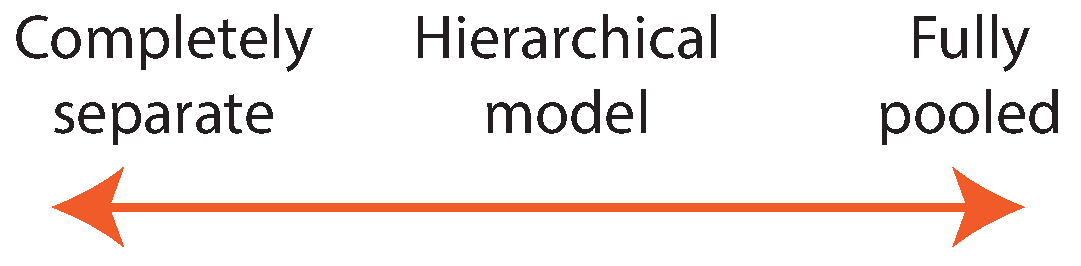
\includegraphics[width=1\textwidth]{figures/lec6_hierarchicalConcept.pdf}}
	\end{figure}
	
\end{frame}

\begin{frame}
	\frametitle{Hierarchical model for EU referendum polls}
	\onslide<2-> As for heterogeneous model we allow $\theta$ to vary by poll:
	
	\onslide<3->
	\begin{equation}
	Pr(X=X_i|\theta_i) = {\theta_i}^{X_i} (1-\theta_i)^{10-X_i}
	\end{equation}
	
	\onslide<4->
	However now we assume that the $\theta_i$ are drawn from a common ``population'' distribution:
	
	\onslide<5->
	\begin{equation}
	\theta_i \sim beta(a,b)
	\end{equation} 
	
	\onslide<6-> where $a$ and $b$ are parameters that define the population-level beta distribution.
	
\end{frame}

\begin{frame}
	\frametitle{Hierarchical model for EU referendum polls}
	
	\begin{figure}[ht]
		\centerline{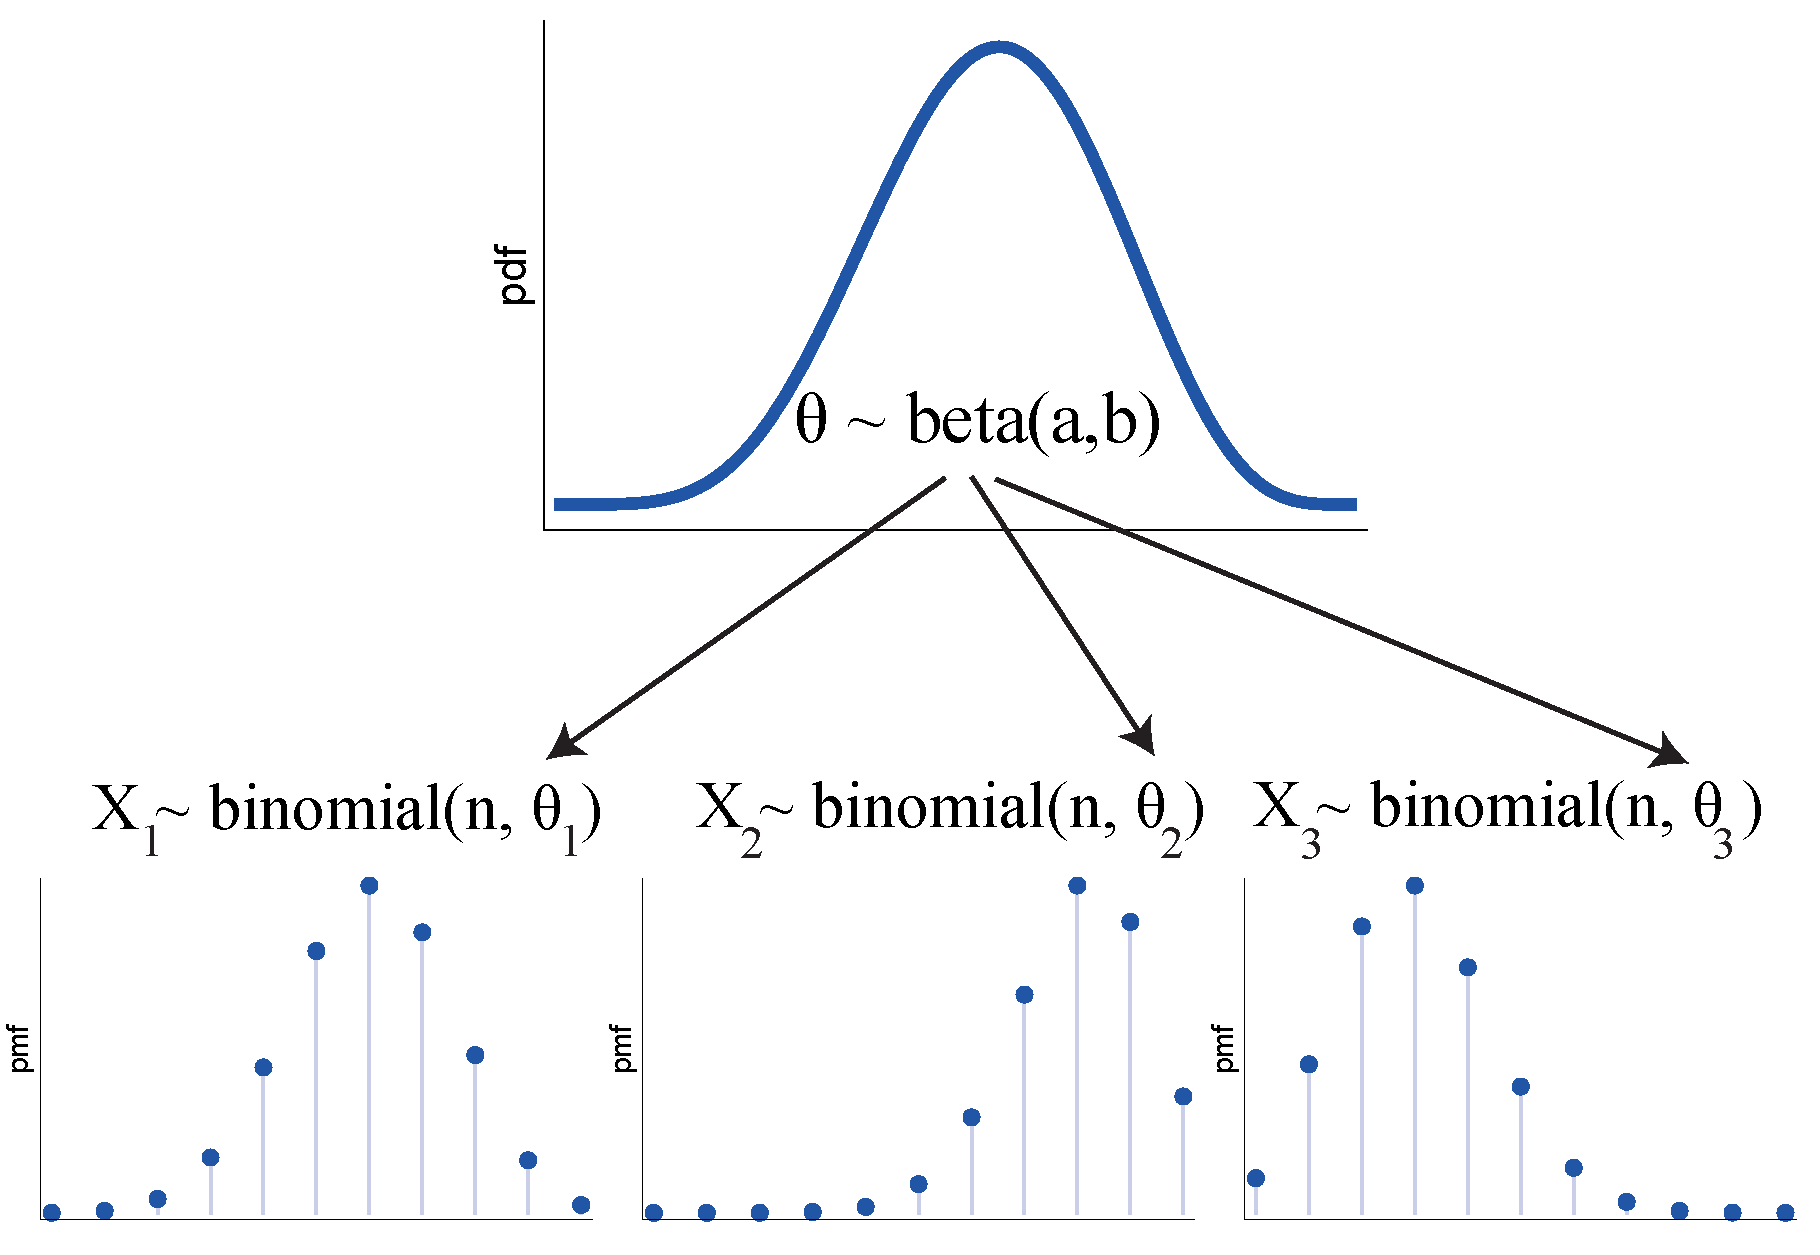
\includegraphics[width=1\textwidth]{figures/lec6_hierarchyConcept.pdf}}
	\end{figure}
	
\end{frame}

\begin{frame}
	\frametitle{Hierarchical model for EU referendum polls}
	\begin{equation}
	\theta_i \sim beta(a,b)
	\end{equation} 
	
	\onslide<2-> $(a,b)$ are parameters just like any other in Bayesian inference $\implies$ assign them \textbf{priors}!
	
	\onslide<3-> Actually easier to set priors for transformed parameters:
	
	\onslide<4-> 
	\begin{align*}
	a &= \alpha \times \kappa\\
	b &= (1-\alpha) \times \kappa
	\end{align*}
	
	\onslide<5-> where $\alpha$ represents the ``population'' chance of voting 'remain' and $\kappa$ measures the concentration $\implies$
	
	\onslide<6->
	\begin{equation}
	\theta_i \sim beta(\alpha \times \kappa,(1-\alpha) \times \kappa)
	\end{equation}
	
\end{frame}

\begin{frame}
	\frametitle{Hierarchical model for EU referendum polls}
	
	\begin{equation}
	\theta_i \sim beta(\alpha \times \kappa,(1-\alpha) \times \kappa)
	\end{equation}
	
	\onslide<2-> Set independent priors:
	
	\onslide<3->
	\begin{equation}
	p(\alpha,\kappa) = p(\alpha) \times p(\kappa)
	\end{equation}
	
	\onslide<4->
	\textbf{Question:} what is the numerator of Bayes' rule for this problem? 
	
	\onslide<5-> \textbf{Answer:} the joint distribution of the data $X$ and parameters; i.e. $p(X,\theta,\alpha,\kappa)$
	
	\onslide<6-> \textbf{Another question:} how do we find this here? 	\onslide<6-> \textbf{Another answer:} exploit conditional independence of the problem!
	
\end{frame}

\begin{frame}
	\frametitle{Hierarchical model for EU referendum polls}
	
	\onslide<2-> Start with ``population'' level parameters.
	
	\begin{figure}[ht]
		\centerline{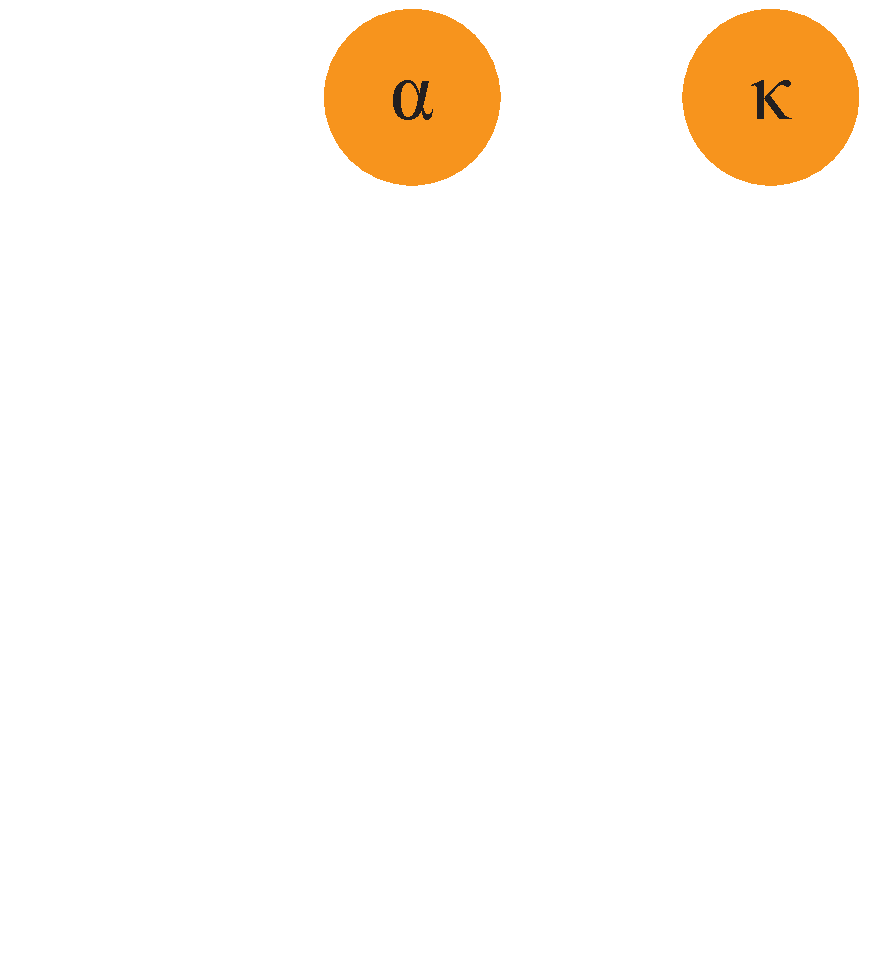
\includegraphics[width=0.6\textwidth]{figures/lec6_conditionalIndependence5.pdf}}
	\end{figure}
	
	
\end{frame}

\begin{frame}
	\frametitle{Hierarchical model for EU referendum polls}
	
	And determine their joint probability.
	
	\begin{figure}[ht]
		\centerline{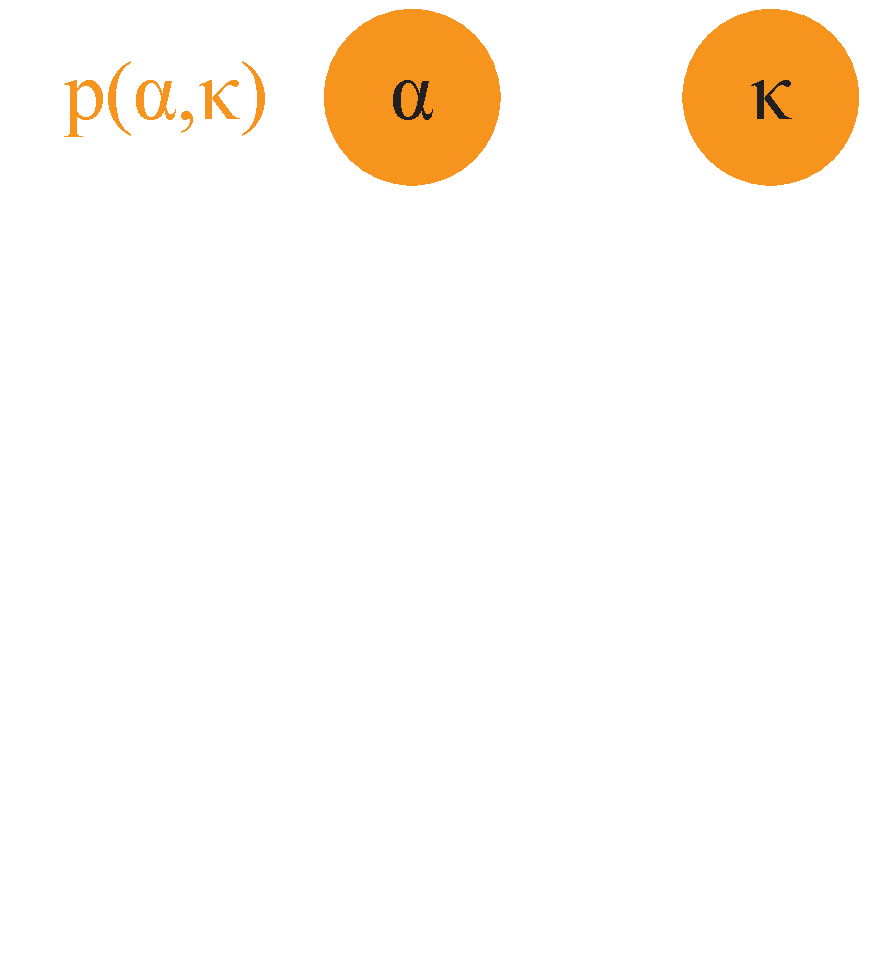
\includegraphics[width=0.6\textwidth]{figures/lec6_conditionalIndependence4.pdf}}
	\end{figure}
	
\end{frame}

\begin{frame}
	\frametitle{Hierarchical model for EU referendum polls}
	
	Find the probability of $\theta$ \textbf{conditional} on $\alpha$ and $\kappa$.
	
	\begin{figure}[ht]
		\centerline{\includegraphics[width=0.6\textwidth]{figures/lec6_conditionalIndependence3.pdf}}
	\end{figure}
	
\end{frame}

\begin{frame}
	\frametitle{Hierarchical model for EU referendum polls}
	
	Find the probability of X \textbf{conditional} on $\theta$ .
	
	\begin{figure}[ht]
		\centerline{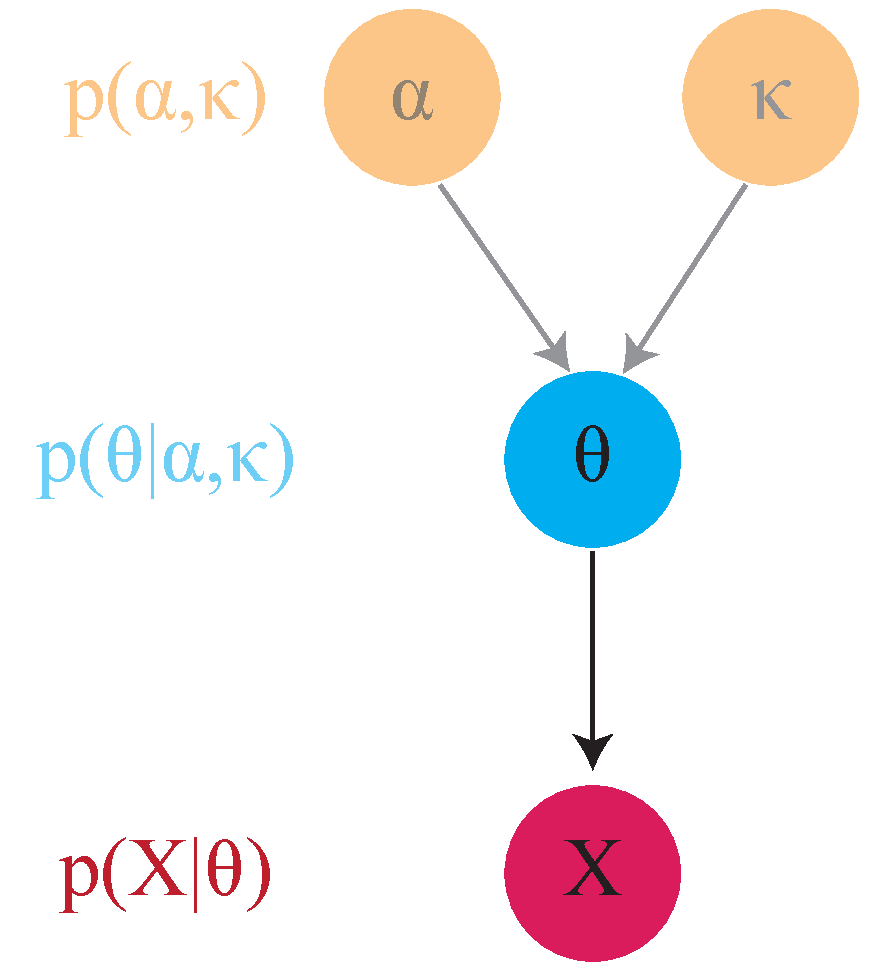
\includegraphics[width=0.6\textwidth]{figures/lec6_conditionalIndependence2.pdf}}
	\end{figure}
	
\end{frame}

\begin{frame}
	\frametitle{Hierarchical model for EU referendum polls}
	
	Finally to obtain the overall probability...
	
	\begin{figure}[ht]
		\centerline{\includegraphics[width=0.6\textwidth]{figures/lec6_conditionalIndependence1.pdf}}
	\end{figure}
	
\end{frame}

\begin{frame}
	\frametitle{Hierarchical model for EU referendum polls}
	
	...multiply together all the terms.
	
	\begin{figure}[ht]
		\centerline{\includegraphics[width=0.6\textwidth]{figures/lec6_conditionalIndependence0.pdf}}
	\end{figure}
	
\end{frame}

\begin{frame}
	\frametitle{Hierarchical model for EU referendum polls}
	\onslide<2-> So the posterior is found as:
	
	\onslide<3->
	\begin{align*}
	p(\theta,\alpha,\kappa|X) &\propto p(X,\theta,\alpha,\kappa)\\
	&= \underbrace{\textcolor{pinkBright}{p(X|\theta)}}_{\text{likelihood}} \times \underbrace{\textcolor{blueBright}{p(\theta|\alpha,\kappa)}}_{\text{prior}} \times \underbrace{\textcolor{orangeBright}{p(\alpha,\kappa)}}_{\text{hyper-prior}}
	\end{align*}
	
	\begin{itemize}
		\item<4-> $\textcolor{pinkBright}{p(X|\theta)}$ is just the \textbf{likelihood}.
		\item<5-> $\textcolor{blueBright}{p(\theta|\alpha,\kappa)}$ is the \textbf{prior} on $\theta$.
		\item<6-> $\textcolor{orangeBright}{p(\alpha,\kappa)}$ is the \textbf{hyper-prior} on the \textbf{hyper-parameters} $\alpha$ and $\kappa$.
		\item<7-> However the word ``hyper'' is really just a fancy word we use to represent priors on ``population'' level parameters.
		\item<8-> In hierarchical models there is a blurring of the likelihood/prior boundary.
	\end{itemize}
	
\end{frame}

\begin{frame}
	\frametitle{Hierarchical model for EU referendum polls: back to the problem}
	\onslide<2-> We set the following independent (hyper-)priors on $\alpha$ and $\kappa$:
	
	\onslide<3->
	\begin{align*}
	\alpha &\sim beta(5,5)\\
	\kappa &\sim pareto(1,0.3)
	\end{align*} 
	
	\onslide<4-> where:
	
	\begin{itemize}
		\item[-]<5-> beta(5,5) has a mean of 0.5, and only has support for $0\leq\alpha\leq 1$.
		\item[-]<6-> pareto(1,0.3) is a distribution only with support for values of $\kappa\geq 1$. 
	\end{itemize}
	
\end{frame}

\begin{frame}[fragile]
	\frametitle{Hierarchical model for EU referendum polls: coding up model in Stan}
	
	\begin{minted}{stan}
parameters {
  real<lower=0, upper=1> alpha;
  real<lower=1> kappa; 
  vector<lower=0, upper=1>[K] theta; 
} 
model {
  for (i in 1:K){
    Y[i] ~ binomial(N[i],theta[i]); // likelihood
  }  
  // prior
  theta ~ beta(alpha * kappa, (1 - alpha) * kappa); 

  // hyper-priors
  kappa ~ pareto(1, 0.3);
  alpha ~ beta(5,5);
}
	\end{minted}
	
\end{frame}

\begin{frame}[fragile]
	\frametitle{Hierarchical model for EU referendum polls: heterogeneous model estimates}
	\onslide<2-> Remember the posterior from the heterogeneous model?
	\onslide<3->
	\begin{figure}[ht]
		\centerline{\includegraphics[width=1\textwidth]{figures/lec6_euHeteroPosterior.pdf}}
	\end{figure}
	
\end{frame}

\begin{frame}[fragile]
	\frametitle{Hierarchical model for EU referendum polls: hierarchical model estimates}
	\onslide<1-> Hierarchical model estimates.
	
	\begin{figure}[ht]
		\centerline{\includegraphics[width=1\textwidth]{figures/lec6_euHierarchicalPosterior.pdf}}
	\end{figure}
	
\end{frame}

\begin{frame}[fragile]
	\frametitle{Hierarchical model for EU referendum polls: hierarchical model estimates}
	\onslide<2-> Two effects evident:
	
	\begin{itemize}
		\item[-]<3-> Shrinkage to \textbf{grand} mean.
		\item[-]<4-> Shrinkage in variance.
	\end{itemize}
	
	\onslide<5-> Shrinkage to grand mean because hierarchical models lie on a spectrum between completely heterogeneous estimates and fully pooled.
	
	\onslide<6->
	\textbf{Important:} the data determine where on the spectrum we exactly end up, so less choice in analysis.
	
	\onslide<7->
	\textbf{Important:} shrinkage helps reduce the variance of estimates $\implies$ outliers have less impact.
	
	\vspace{0.2cm}
	
	\onslide<8->
	Also ``partially-pooling'' information across groups $\implies$ essentially a larger sample size and lower variance. 
	
	
\end{frame}

\begin{frame}
	\frametitle{Hierarchical model: forecasting outcome of overall elections}
	\onslide<2-> Want to estimate the value of $\theta$ for the last poll: the referendum itself.

 \vspace{0.5cm}
	
	\onslide<3-> To do this do the following:
	
	\begin{enumerate}
		\item<4-> Sample $(\alpha,\kappa)$ from their posteriors.
		\item<5-> Sample $\theta\sim beta(\alpha\kappa,(1-\alpha)\kappa)$.
	\end{enumerate}
	
\end{frame}

\begin{frame}
	\frametitle{Hierarchical model: forecasting outcome of overall elections}
	\onslide<2-> Yields the posterior below (gulp):
	
	\onslide<3->
	\begin{figure}[ht]
		\centerline{\includegraphics[width=1\textwidth]{figures/lec6_euOverallThetaPost.pdf}}
	\end{figure}
	
\end{frame}

\begin{frame}
	\frametitle{Hierarchical model: forecasting outcome of overall elections}
	Conclusion: the result could go either way.
	
	\begin{figure}[ht]
		\centerline{\includegraphics[width=1\textwidth]{figures/lec6_euOverallThetaPost.pdf}}
	\end{figure}
	
\end{frame}

\begin{frame}
	\frametitle{Hierarchical models: summary}
	\begin{itemize}
		\item<2-> Model with \textbf{same} parameters for all groups $\implies$ data generating process is the \textbf{same}.
		\item<3-> Model with separately estimated group-level parameters $\implies$ data generating process is completely \textbf{different}.
		\item<4-> Frequently neither of the aforementioned models are appropriate; i.e. we want some dependence between parameters but not 100\%.
		\item<5-> $\implies$ use hierarchical model where the data determines parameter dependence across groups.
		\item<6-> In hierarchical models $\implies$ \textbf{shrinkage} of \textbf{group} means towards the \textbf{grand} mean.
		\item<7-> Also \textbf{shrinkage }of group variance $\impliedby$ sample size$\uparrow$ by \textbf{partial-pooling} information across groups.
	\end{itemize}
\end{frame}

\section{Ordinary differential equations}
\frame{\tableofcontents[currentsection]}

\begin{frame}
	\frametitle{Example: bacterial growth}
	\begin{itemize}
		\item<2-> We carry out experiments where we inoculate agar plates with bacteria at time 0.
		\item<3-> At pre-defined time intervals we count the number of bacteria on each plate, $N(t)$.
		\item<4-> Suppose we want to model bacterial population growth over time.
	\end{itemize}
	
	\onslide<1->
	\begin{figure}[ht]
		\centerline{\includegraphics[width=1\textwidth]{figures/bacteria.png}}
	\end{figure}
	
\end{frame}

\begin{frame}
	\frametitle{Example: bacteria growth data}
	
	\begin{figure}[ht]
		\centerline{\includegraphics[width=1\textwidth]{figures/lec7_odeSingle.pdf}}
	\end{figure}
	
\end{frame}

\begin{frame}
	\frametitle{Example: bacterial growth model}
	\begin{itemize}
		\item<2-> Assume the following model for bacterial population growth:
	\end{itemize}
	
	\onslide<3->
	\begin{equation}
	\frac{\mathrm{d}N}{\mathrm{d}t} = \alpha N (1-\beta N)
	\end{equation}
	
	\onslide<4->
	where $\alpha>0$ is the rate of growth due to bacterial cell division, and $\beta>0$ measures the reduction in growth rate due to ``crowding''. 
	
	\onslide<5->
	\textbf{Question:} how should we infer the parameters of this model?
	
\end{frame}

\begin{frame}
	\frametitle{Example: bacterial growth model}
	\onslide<2->
	\textbf{Answer:} assume measurement error around true value:
	
	\onslide<3->
	\begin{equation}
	N^*(t) \sim \text{normal}(N(t), \sigma)
	\end{equation}

\onslide<4->
where
\begin{itemize}
	\item<5-> $N^*(t)$ is the \textbf{measured} count of bacteria at time $t$.
	\item<6-> $N(t)$ is the solution to the ODE at time $t$ (true number of bacteria on plate.)
	\item<7-> $\sigma>0$ measures the magnitude of the measurement error about the true value.
\end{itemize}

\onslide<8-> \textbf{Question:} how does this model work?

\end{frame}

\begin{frame}
	\frametitle{Example: bacterial growth model}
	Start with true number of bacterial cells, $N(t)$.
	
	\onslide<2->
		\begin{figure}[ht]
			\centerline{\includegraphics[width=1\textwidth]{figures/lec7_odeSingleBulding1.pdf}}
		\end{figure}
	
\end{frame}

\begin{frame}
	\frametitle{Example: bacterial growth model}
	Overlay sampling distribution representing measurement error.
	
	\begin{figure}[ht]
		\centerline{\includegraphics[width=1\textwidth]{figures/lec7_odeSingleBulding2.pdf}}
	\end{figure}
	
\end{frame}

\begin{frame}
	\frametitle{Example: bacterial growth model}
	And data generated from this process.
	
	\begin{figure}[ht]
		\centerline{\includegraphics[width=1\textwidth]{figures/lec7_odeSingleBulding3.pdf}}
	\end{figure}
	
\end{frame}

\begin{frame}
	\frametitle{Example: bacteria growth model inference}
	\onslide<2-> Remember we are using a normal likelihood:
	
	\onslide<3->
	\begin{equation}
	N^*(t) \sim \text{normal}(N(t), \sigma)
	\end{equation}
	
	\onslide<4->
	$\implies$ likelihood for all observations:
	
	\onslide<5->
	\begin{equation}
	L(N(t),\sigma) = \prod_{t={t_1}}^{T} \frac{1}{\sqrt{2\pi\sigma^2}} exp\left[\frac{-(N^*(t) - N(t))^2}{2\sigma}\right]
	\end{equation}
	
	\onslide<6->
	\textbf{Question:} how do we calculate $N(t)$?
	
\end{frame}

\begin{frame}
	\frametitle{Example: bacteria growth model inference}
	
	\begin{equation}
	\frac{\mathrm{d}N}{\mathrm{d}t} = \alpha N (1-\beta N)
	\end{equation}
	
	\begin{itemize}
		\item<2-> In most ODE models, the mean $N(t)$ cannot be solved for exactly so we \textbf{can't write down a ``closed-form'' expression for the likelihood.}
		\item<3-> $\implies$ approximate answer using a numerical method.
		\item<4-> However any solution for $N(t)$ - exact or numerical - depends on the parameters of the ODE model. For our example:
		
		\onslide<5->
		
		\begin{equation}
		N(t) = f(t,\alpha,\beta)
		\end{equation}
		
	\end{itemize}
	
	\vspace{0.2cm}
	
	\onslide<6->
	\textbf{Question:} how do we do MCMC in this setting?
	
\end{frame}

\begin{frame}
	\frametitle{Example: bacteria growth model inference}
	
	\onslide<2-> For example, in Random Walk Metropolis:
	
	\begin{itemize}
		\item<3-> Start at random location in $(\alpha,\beta,\sigma)$ space.
		\item<4-> For t=1,...,T do:
		\begin{enumerate}
			\item<5-> Propose a new location $(\alpha',\beta',\sigma')$ using a jumping distribution.
			\item<6-> Numerically (or analytically) integrate ODE to solve for $N(t,\alpha',\beta')$.
			\item<7-> Calculate un-normalised posterior at proposed location $\implies$ calculate $r$.
			\item<8-> Based on $r$ move to new location or stay at original.
		\end{enumerate}
	\end{itemize}

	\onslide<9->
	$\implies$ at every step we must solve ODE for $N(t)$; can be computationally expensive!
	
\end{frame}

\begin{frame}[fragile]
	\frametitle{Example: bacteria growth model in Stan}
	\begin{itemize}
		\item<2-> ODE models can be slow to converge - particularly when accounting for numerical solution of equations.
		\item<3-> Fortunately Stan has an inbuilt ODE integrator $\implies$ can leverage the speed of HMC (NUTS) for ODE systems!
		\item<4-> Write a function that returns the derivative (RHS of ODE):
		\onslide<5->
\begin{minted}{stan}
real[] bacteria_diff(real t,real[] N,
              real[] theta,real[] x_r,int[] x_i){
  real dNdt[1];
  dNdt[1] <- theta[1] * N[1] * 
                     (1 - theta[2] * N[1]);
  return dNdt;
}
\end{minted}
		
	\end{itemize}
	
	
\end{frame}

\begin{frame}[fragile]
	\frametitle{Example: bacteria growth model in Stan}
	
\begin{minted}{stan}
model {
    sigma ~ cauchy(0,1); // Prior
    theta ~ normal(0,2); // Prior for alpha, beta
    N0 ~ normal(5,2); // Prior
    
    // Solve ODE at current parameter values
    real N_hat[T,1];
    N_hat <- integrate_ode_rk45(bacteria_diff, N0, t0, ts, 
                    theta, x_r, x_i);
    // Likelihood
    for (t in 1:T) {
        N[t] ~ normal(N_hat[t,1],sigma);
     }
}
\end{minted}

\onslide<2->
$\implies$ \mintinline{stan}{integrate_ode} takes the derivative function as its first input argument. 

\end{frame}

\begin{frame}
	\frametitle{Issues with inference for ODEs and PDEs}
	\onslide<2-> Whilst Stan's integrator makes it quite easy to use HMC to do MCMC, there are still problems that arise:
	\begin{itemize}
		\item<3-> ODE models are very often non-identifiable $\implies$ need to reparameterise model.
		\item<4-> (Linked) ODE models can be slower to converge than simpler models $\implies$ need to run MCMC for longer before $\hat{R}<1.1$ achieved.
	\end{itemize}
	
	\onslide<5->
	$\implies$ important that we ``know'' our model well before we start to do inference explicitly.

 \vspace{0.5cm}

 \onslide<7-> Oxford has produced PINTS, which houses many MCMC algorithms which are good for ODE-type models.
	
\end{frame}


\begin{frame}
	\frametitle{Inference for ODEs: summary}
	\begin{itemize}
		\item<2-> ODE models are no harder to formulate than ``traditional'' problems.
		\item<3-> However for ODE models we cannot typically write down a ``closed-form'' expression for the likelihood.
		\item<4-> $\implies$ use integrator to numerically solve for mean for each set of parameters.
		\item<5-> Stan has inbuilt integrator meaning we can do MCMC using Stan's fast HMC implementation.
		\item<6-> ODE models are often under-identified $\implies$ do non-linear least squares, or approximate Bayesian computation \textit{before} MCMC.
	\end{itemize}
	
\end{frame}


\section{Model comparison}
\frame{\tableofcontents[currentsection]}

\begin{frame}
	\frametitle{Why do we need a measure of a model's fit?}
	
	\onslide<2->
	Often in modelling we are required to choose between a number of models, in order to:
	
	\begin{itemize}
		\item<3-> Test between rival hypotheses about the real world.
		\item<4-> Choose the most predictive model to make forecasts about the future.
		\item<5-> Avoid the computational expense of using a number of models for some future use.
	\end{itemize}
	
	\onslide<6-> \textbf{Note:} model selection can sometimes be avoided by \textbf{a.} using a parameter to specify model choice or \textbf{b.} using a general model that allows all models as special cases.
	
\end{frame}

\begin{frame}
	\frametitle{Which of these models is more predictive?}
	
	\begin{figure}[ht]
		\centerline{\includegraphics[width=0.95\textwidth]{figures/lec7_modelFitTest.pdf}}
	\end{figure}

\end{frame}

\begin{frame}
	\frametitle{Simple models generalise better to out-of-sample data}

	\begin{figure}[ht]
	\centerline{\includegraphics[width=0.85\textwidth]{figures/lec7_modelFitTest1.pdf}}
\end{figure}

\onslide<2->
$\implies$ right model is \textbf{overfit} to data; it fits the \textbf{noise} not the \textbf{signal}.
	
\end{frame}

\begin{frame}
	\frametitle{Selection bias in model selection}
	
	\onslide<2-> \textbf{The problem:}
	\begin{itemize}
		\item<3-> Want to measure a model's predictive capability on an \textbf{independent} data set; i.e. one that has not been used to fit our model.
		\item<4-> But don't have out-of-sample data! (If we did it would form part of the ``sample''!)
		\item<5-> If use in-sample data to gauge model fitness $\implies$ predictive performance is upwardly-biased due to overfit.
	\end{itemize}
	
	\onslide<6-> 
	\textbf{Note:} this selection bias effect $\implies$ posterior predictive checks will fail to detect model overfit.
	
\end{frame}

\begin{frame}
	\frametitle{Selection bias in model selection}
	\onslide<2-> \textbf{Solutions:}
	
	\begin{itemize}
		\item<3-> Use \textbf{heuristics} to correct in-sample measures of fit to account for overfit.
		\item<4-> (Better)  Use \textbf{cross validation} where data is partitioned into:
		\begin{itemize}
			\item[-]<5-> ``Training'' sets: used to fit model.
			\item[-]<6-> ``Testing'' sets: used to  evaluate model.
		\end{itemize}
	\end{itemize}
	
\end{frame}

\begin{frame}
	\frametitle{Using heuristics to estimate out-of-sample predictive performance}
	
	\onslide<2-> Correct measures of fit to account for overfitting:
	\begin{itemize}
		\item<2-> $R^2\rightarrow \overline{R^2}$; i.e. a metric that measures proportion of variance explained by model.
		\item<3-> $\text{Log-likelihood}\rightarrow$ AIC, DIC, or WAIC; more appropriate metric for Bayesian models due to their basis in likelihood/probability.
	\end{itemize}
	
	\onslide<1->
		\begin{figure}[ht]
			\centerline{\includegraphics[width=0.85\textwidth]{figures/magic.jpg}}
		\end{figure}
	
\end{frame}

\begin{frame}
	\frametitle{Ranking heuristics}
	
	\begin{figure}[ht]
		\centerline{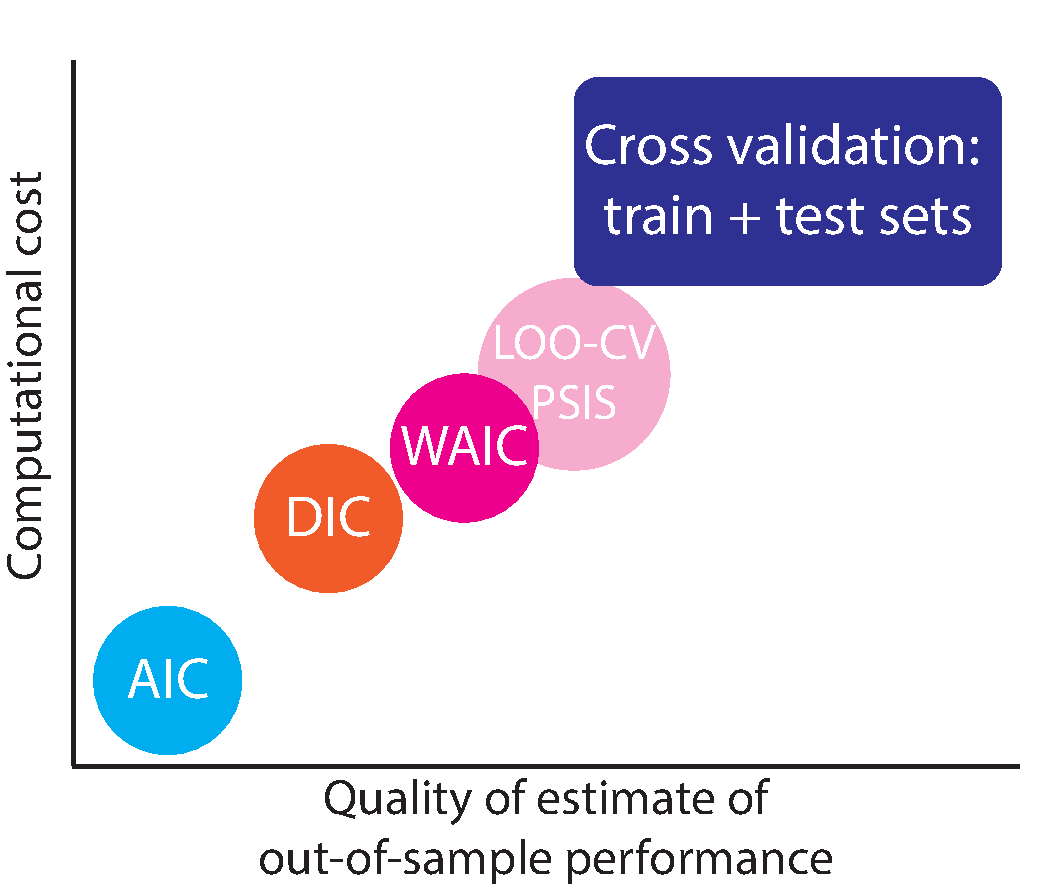
\includegraphics[width=0.85\textwidth]{figures/lec7_conceptMetrics.pdf}}
	\end{figure}
	
\end{frame}

\begin{frame}
	\frametitle{Evaluating heuristics: AIC}
	\onslide<2-> ``Akaike Information Criterion'' computed by (ignoring -2 at front):
	
	\onslide<3->
	\begin{equation}
	\text{AIC} = log \;p(X|\hat{\theta}_{MLE}) - k
	\end{equation}
	
	\onslide<4-> where $k$ is the number of parameters estimated in model fitting, and $\hat{\theta}_{MLE}$ is maximum likelihood (point) estimate.
	
	\begin{itemize}
		\item<5-> Based on asymptotic approximation to normal linear models with uniform priors.
		\item<6-> $\implies$ not reasonable correction for more general models; particularly hierarchical ones.
		\item<7-> Ignores uncertainty in parameter estimates, and hence log-likelihood.
	\end{itemize}

\end{frame}

\begin{frame}
	\frametitle{Evaluating heuristics: DIC}
	\onslide<2-> ``Deviance Information Criterion'' computed by (ignoring -2 at front):
	
	\onslide<3->
	\begin{equation}
	\text{DIC} = log \;p(X|\hat{\theta}_{Bayes}) - p_{DIC}
	\end{equation}
	
	\onslide<4-> where $\hat{\theta}_{Bayes}$ is posterior mean (point) estimate and $p_{DIC}$ is the ``effective number of parameters'' defined by:
	
	\onslide<5->
	\begin{equation}
	p_{DIC} = 2 var_{post} \left[log\; p (X|\theta)\right]
	\end{equation}
	
	\onslide<6->
	which is typically estimated across all posterior samples.
	
	\onslide<7->
	\begin{equation}
	p_{DIC} \approx 2 V_{s=1}^{S}log\; p (X|\theta_s)
	\end{equation}

\end{frame}

\begin{frame}
	\frametitle{DIC complexity correction intuition: complex models have high parameter uncertainty}
	
	\begin{figure}[ht]
		\centerline{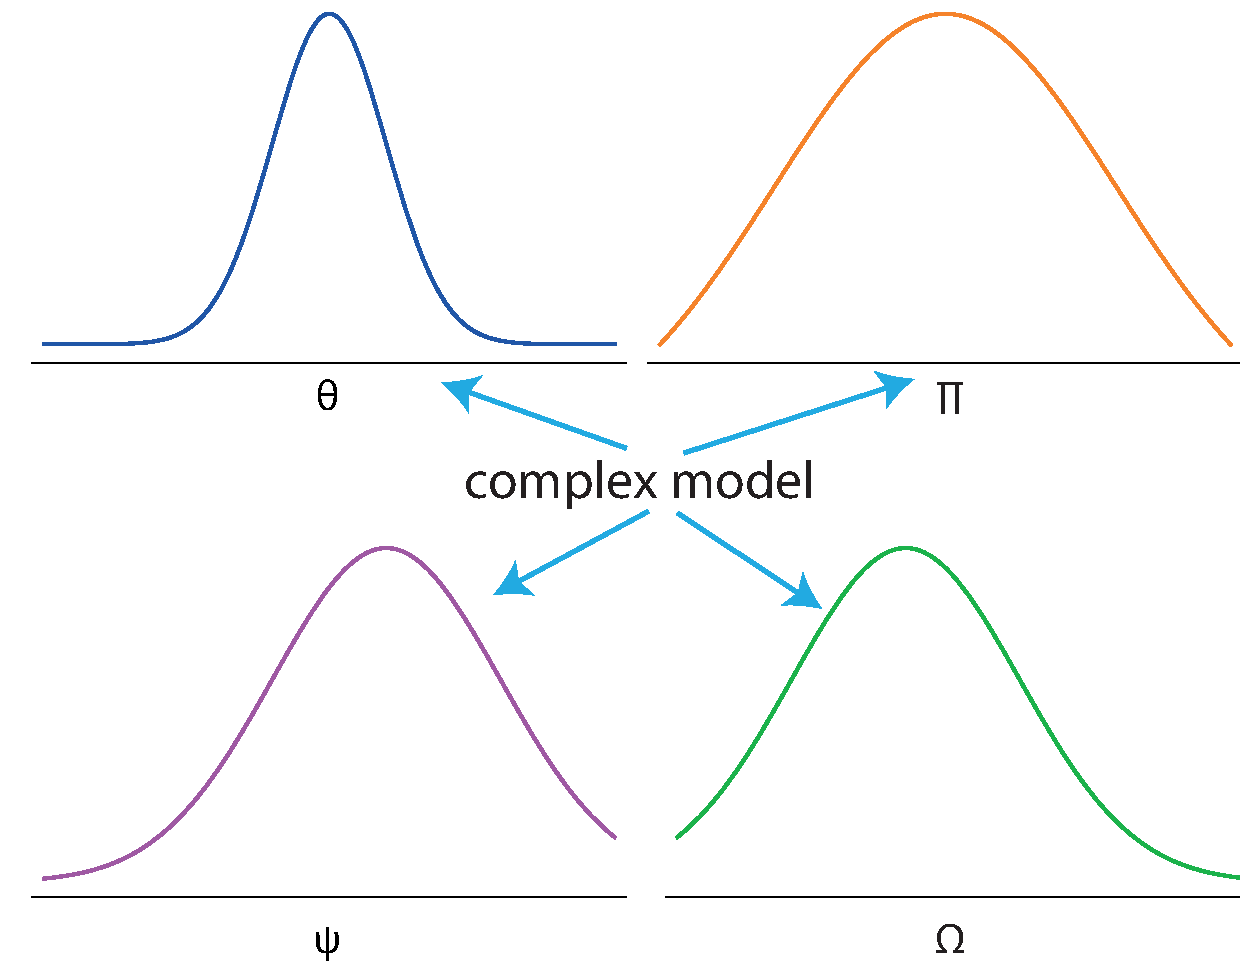
\includegraphics[width=0.9\textwidth]{figures/lec7_overfit.pdf}}
	\end{figure}
	
\end{frame}

\begin{frame}
	\frametitle{DIC complexity correction intuition: simpler models have lower uncertainty}
	
	\begin{figure}[ht]
		\centerline{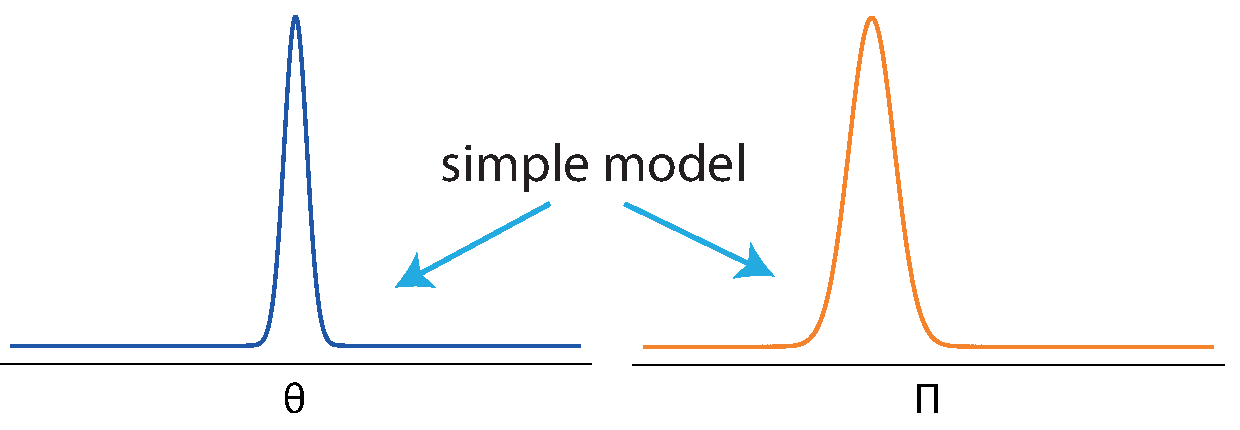
\includegraphics[width=1\textwidth]{figures/lec7_simple.pdf}}
	\end{figure}
	
\end{frame}

\begin{frame}
	\frametitle{DIC complexity correction intuition: lower posterior uncertainty $\implies$ lower uncertainty in fit}
	
	\begin{figure}[ht]
		\centerline{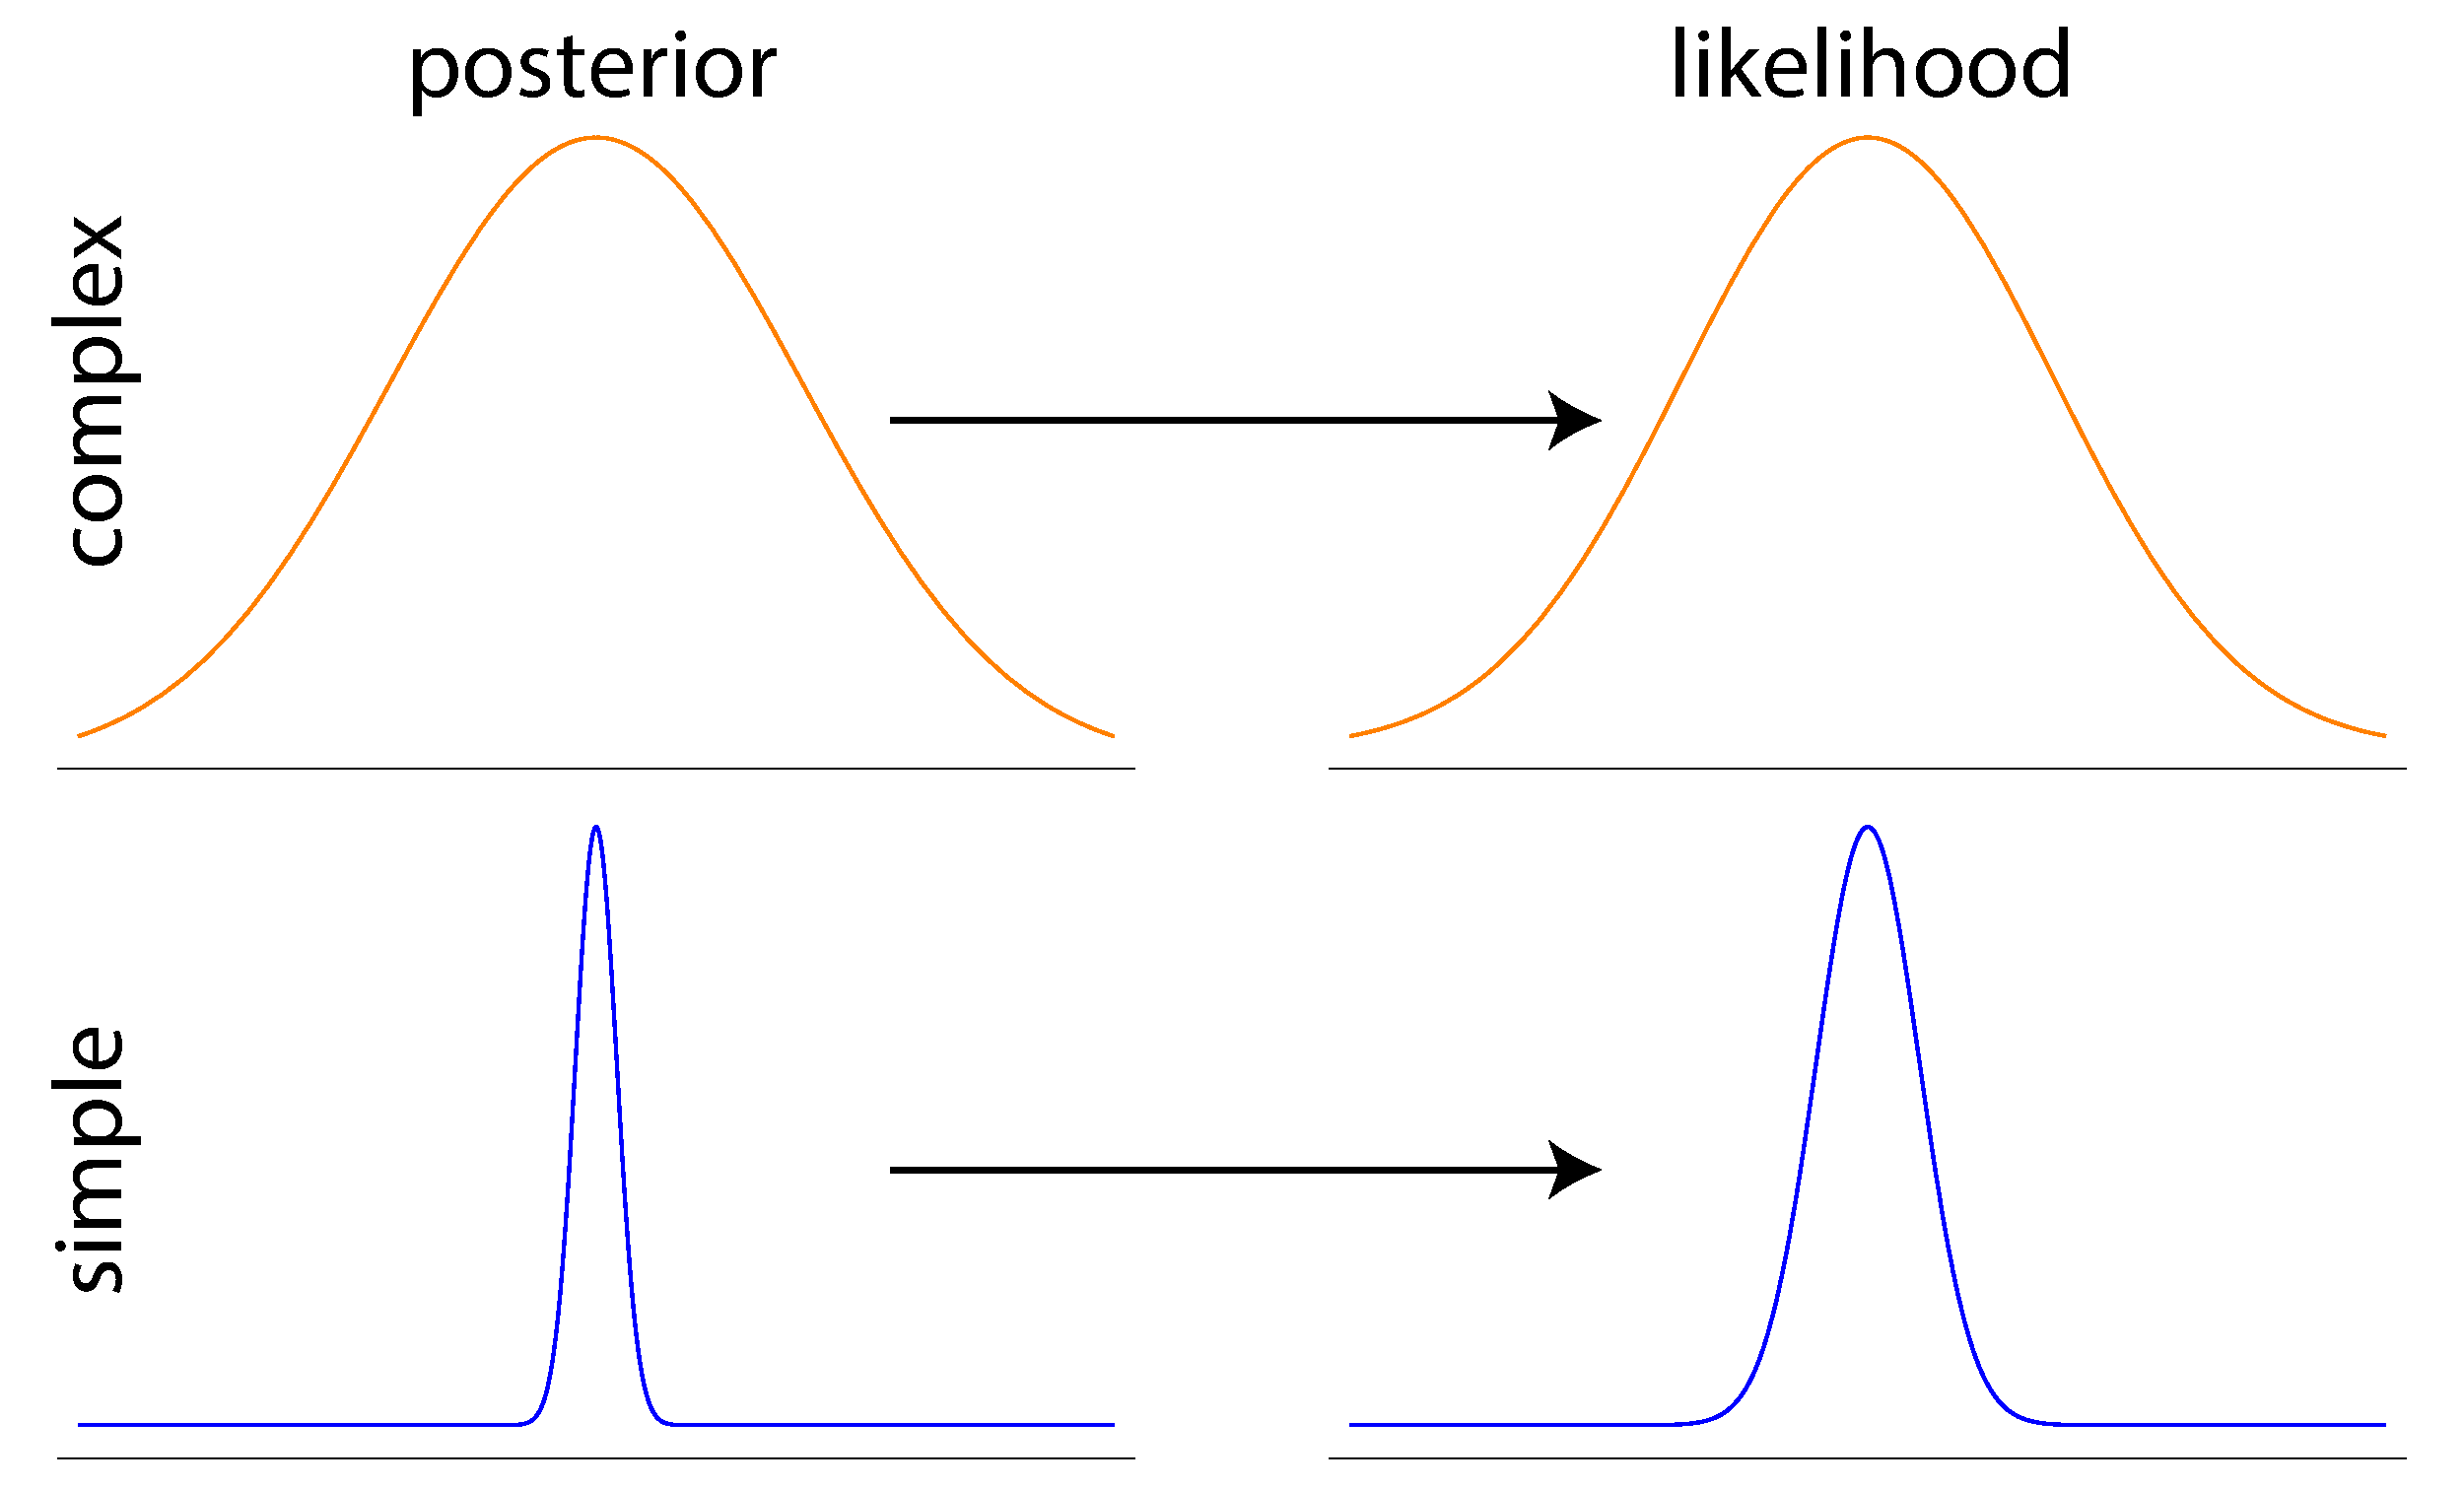
\includegraphics[width=1\textwidth]{figures/lec7_correctionPanel.pdf}}
	\end{figure}
	
\end{frame}

\begin{frame}
	\frametitle{Evaluating heuristics: DIC}
	\begin{equation}
	p_{DIC} = 2 var_{post} \left[log\; p (X|\theta)\right]
	\end{equation}
	
	\begin{itemize}
		\item<2-> Spiegalhalter (2002) introduced $P_{DIC}$ as a measure of model dimensionality.
		\item<3-> Overfit models have many parameters, each with high uncertainty.
		\item<4-> A high variance in $\theta$ $\implies$ high variance in $log(X|\theta)$.
		\item<5-> $\implies$ $p_{DIC}$ is big, so large correction.
	\end{itemize}
	
\end{frame}

\begin{frame}
	\frametitle{DIC issue: uses a point estimate to determine fit}
	
		\begin{figure}[ht]
			\centerline{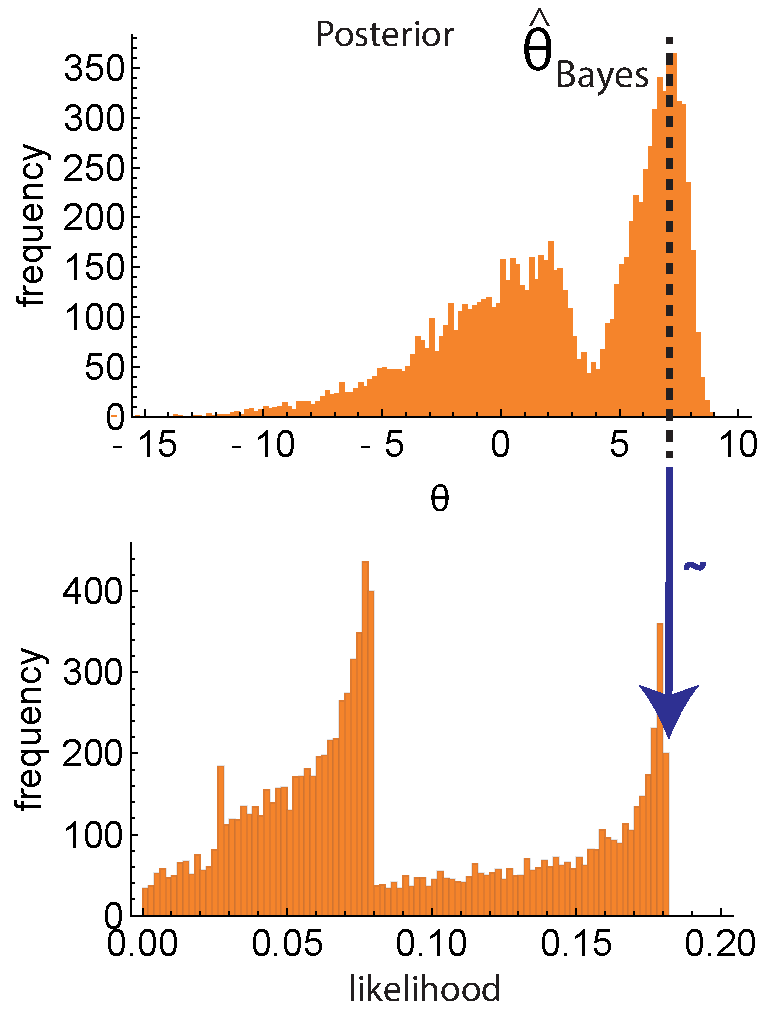
\includegraphics[width=0.55\textwidth]{figures/lec7_likelihood1.pdf}}
		\end{figure}
	
\end{frame}

\begin{frame}
	\frametitle{Evaluating heuristics: DIC}
	\begin{equation}
	\text{DIC} = log \;p(X|\hat{\theta}_{Bayes}) - p_{DIC}
	\end{equation}

\onslide<2-> In summary:

\begin{itemize}
	\item<3-> Uses less arbitrary notion of model dimensionality to correct measure of fit than AIC.
	\item<4-> $\implies$ better for a wider class of models.
	\item<5-> Still does not fully address uncertainty in fit since calculates first term above with a point estimate $\hat{\theta}_{Bayes}$.
\end{itemize}

\end{frame}

\begin{frame}
	\frametitle{Evaluating heuristics: WAIC}
	\onslide<2-> ``Watanabe-Akaike Information Criterion'' (Watanabe, 2010) computed by (ignoring -2 at front):
	
	\onslide<3->
	\begin{equation}
	WAIC = \underbrace{\sum_{i=1}^{N} log\left(\frac{1}{S}\sum_{s=1}^{S} p(X_i|\theta_s)\right)}_{\text{log pointwise predictive density}} - p_{WAIC}
	\end{equation}
	
	\onslide<4-> Since allows for uncertainty in fit $\implies$ fully Bayesian estimate.
	
	\onslide<5-> Where $p_{WAIC}$ is another correction factor calculated by:
	
	\onslide<6->
	\begin{equation}
	p_{WAIC} = \sum_{i=1}^{N} var_{post} \left[log\; p(X_i|\theta)\right]
	\end{equation}
	
\end{frame}

\begin{frame}
	\frametitle{WAIC: averages likelihood over posterior to determine fit}
	
	\begin{figure}[ht]
		\centerline{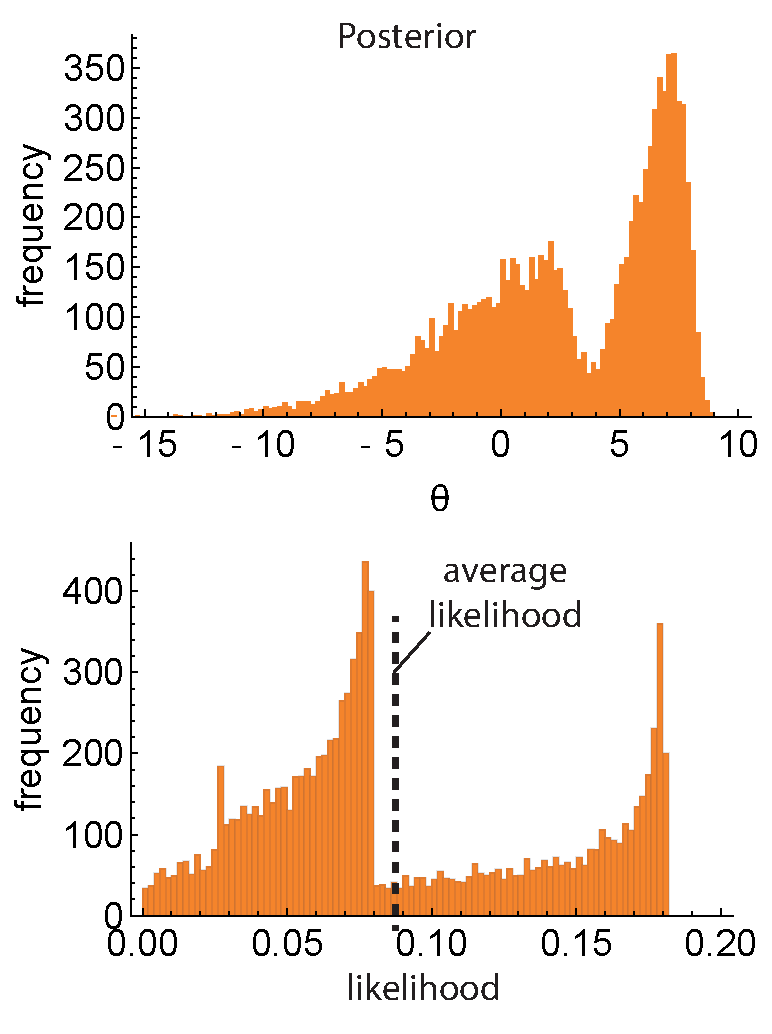
\includegraphics[width=0.55\textwidth]{figures/lec7_likelihood2.pdf}}
	\end{figure}
	
\end{frame}


\begin{frame}
	\frametitle{Evaluating heuristics: WAIC}
	\begin{equation}
	WAIC = \underbrace{\sum_{i=1}^{N} log\left(\frac{1}{S}\sum_{s=1}^{S} p(X_i|\theta_s)\right)}_{\text{log pointwise predictive density}} - \sum_{i=1}^{N} var_{post} \left[log\; p(X_i|\theta)\right]
	\end{equation}
	
	\onslide<2->
	In summary:
	
	\begin{itemize}
		\item<3-> Fully Bayesian since estimates fit across all posterior samples.
		\item<4-> Evaluates the log predictive density using pointwise sums.
		\item<5-> $\implies$ for structured models can be problematic if model not easily split into parts (can always use groups rather than individual points, though.)
		\item<6-> (Still an \textbf{approximation} $\implies$ ideally use proper cross validation.)
	\end{itemize}
	
\end{frame}

\begin{frame}[fragile]
	\frametitle{WAIC using Stan + `loo' package}
	\onslide<2-> Use ``generated quantities'' block to store log-likelihood across all data points. For example:
	
	\onslide<3->
\begin{minted}{stan}
model {
    ...
   for (i in 1:N){
      y[i] ~ normal(mu,sigma);
    }
}
generated quantities{
    vector logLikelihood[N];
    for (i in 1:N){
       logLikelihood[i] <- normal_log(y[i],mu,sigma);
    }
}
\end{minted}
	
\end{frame}

\begin{frame}[fragile]
	\frametitle{WAIC using Stan + `loo' package}
	\begin{knitrout}
		\small
		\definecolor{shadecolor}{rgb}{0.969, 0.969, 0.969}\color{fgcolor}\begin{kframe}
			\begin{alltt}
				\hlkwd{library}\hlstd{(loo)}
			\end{alltt}
			\begin{alltt}
				\hlcom{## Extract log-likelihood}
				\hlstd{logLikelihood} \hlkwb{<-} \hlkwd{extract_log_lik}\hlstd{(fit,}\hlstr{'logLikelihood'}\hlstd{)}
				
				\hlcom{## Calculate WAIC}
				\hlstd{aWAIC} \hlkwb{<-} \hlkwd{waic}\hlstd{(logLikelihood)}
				
				\hlcom{## Print answer}
				\hlkwd{print}\hlstd{(aWAIC)}
			\end{alltt}
			\begin{verbatim}
			## Computed from 12000 by 5000 log-likelihood matrix
			## 
			##           Estimate   SE
			## elpd_waic -10543.1 49.9
			## p_waic         4.0  0.1
			## waic       21086.3 99.7
			\end{verbatim}
		\end{kframe}
	\end{knitrout}
\end{frame}

\begin{frame}[fragile]
	\frametitle{``loo'' also estimates leave-one-out-cross-validation errors using importance sampling}
	\begin{knitrout}
		\footnotesize
		\definecolor{shadecolor}{rgb}{0.969, 0.969, 0.969}\color{fgcolor}\begin{kframe}
			\begin{alltt}
				\hlcom{## Estimate LOO-CV}
				\hlstd{aLOO} \hlkwb{<-} \hlkwd{loo}\hlstd{(logLikelihood)}
				
				\hlcom{## Print answer}
				\hlkwd{print}\hlstd{(aLOO)}
			\end{alltt}
			\begin{verbatim}
			## Computed from 12000 by 5000 log-likelihood matrix
			## 
			##          Estimate   SE
			## elpd_loo -10543.1 49.9
			## p_loo         4.0  0.1
			## looic     21086.3 99.7
			## 
			## All Pareto k estimates OK (k < 0.5)
			\end{verbatim}
		\end{kframe}
	\end{knitrout}
	
	\onslide<2->
	\textbf{Note:} this is a preferred measure to WAIC, but be careful $\implies$ if get Pareto k estimates warning do manual cross validation.
	
\end{frame}


\begin{frame}[fragile]
	\frametitle{Important: use pairwise comparison to do model selection with WAIC or LOO-CV}
	\begin{knitrout}
		\footnotesize
		\definecolor{shadecolor}{rgb}{0.969, 0.969, 0.969}\color{fgcolor}\begin{kframe}
			\begin{alltt}
				\hlcom{## Extract log-likelihood for both models}
				\hlstd{logLikelihood_1} \hlkwb{<-} \hlkwd{extract_log_lik}\hlstd{(fit_1,}\hlstr{'logLikelihood'}\hlstd{)}
				\hlstd{logLikelihood_2} \hlkwb{<-} \hlkwd{extract_log_lik}\hlstd{(fit_2,}\hlstr{'logLikelihood'}\hlstd{)}
				
				\hlcom{## Estimate LOO-CV for eac}
				\hlstd{aLOO_1} \hlkwb{<-} \hlkwd{loo}\hlstd{(logLikelihood_1)}
				\hlstd{aLOO_2} \hlkwb{<-} \hlkwd{loo}\hlstd{(logLikelihood_2)}
				
				\hlcom{## Print answer}
				\hlkwd{compare}\hlstd{(aLOO_1,aLOO_2)}
			\end{alltt}
			\begin{verbatim}
			## elpd_diff        se 
			##      -0.7       0.7
			\end{verbatim}
		\end{kframe}
	\end{knitrout}
	\onslide<2->
	$\implies$ pairwise comparison takes a proper account of uncertainty in fit of each model \textbf{relative} to the other.
\end{frame}

\begin{frame}
	\frametitle{Manual cross-validation}
	\begin{itemize}
		\item<2-> The aforementioned methods \textbf{approximate} out-of-sample predictive capability by use of post-hoc corrections to account for overfitting.
		\item<3-> A better class of approximations is to partition the dataset and do proper \textbf{cross-validation.}
	\end{itemize}
	
	\onslide<4->
	\textbf{Question:} how should we choose our training and test sets?
	
\end{frame}

\begin{frame}
	\frametitle{Manual cross-validation: leave-one-out cross-validation}
	
	\begin{figure}[ht]
		\centerline{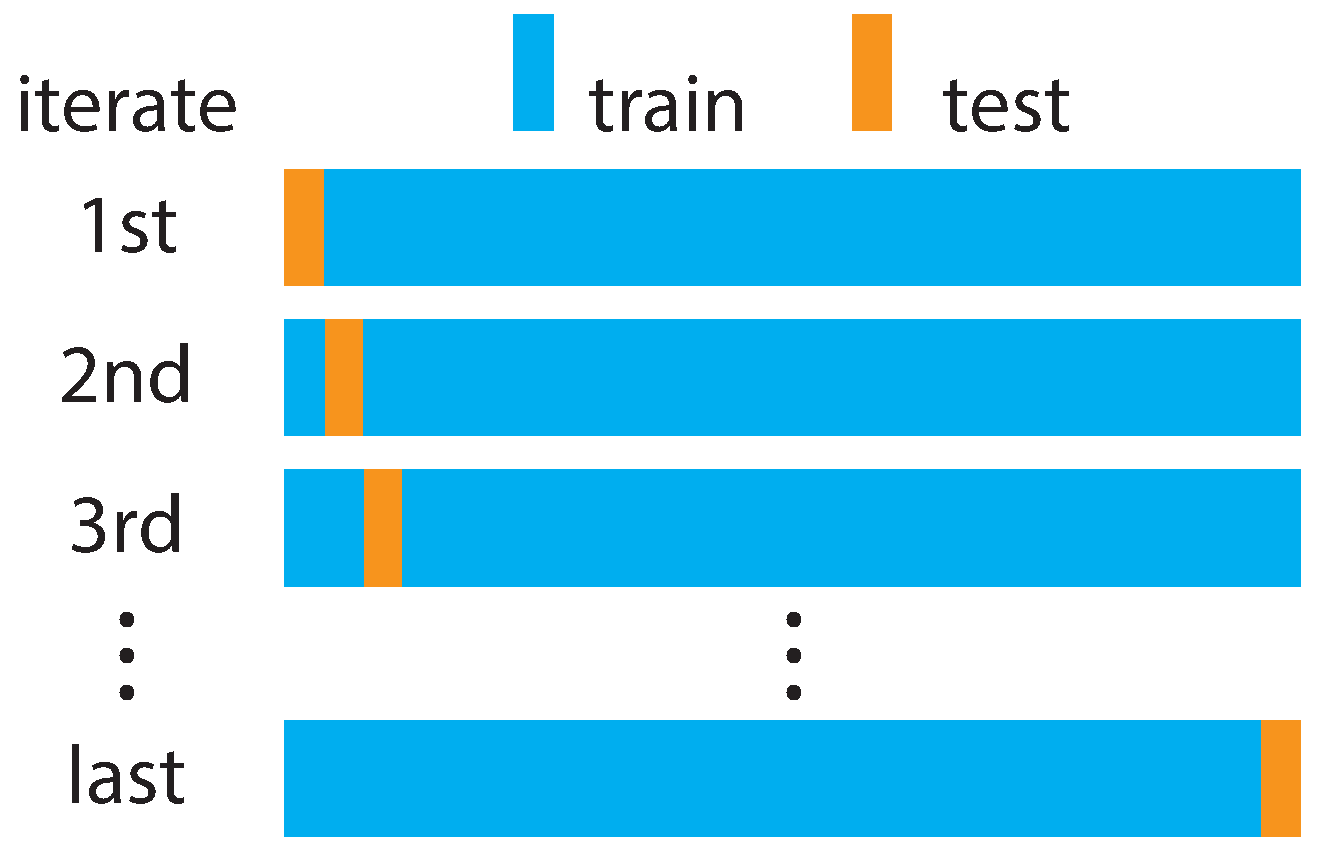
\includegraphics[width=0.8\textwidth]{figures/lec7_testSet_loo.pdf}}
	\end{figure}
	
	\onslide<2->
	$\implies$ average log-likelihood across all posterior $\theta$ across all partitions. \textbf{Note:} no need for overfitting correction!
	
\end{frame}

\begin{frame}
	\frametitle{Manual cross-validation: k-fold cross-validation}
	
	\begin{figure}[ht]
		\centerline{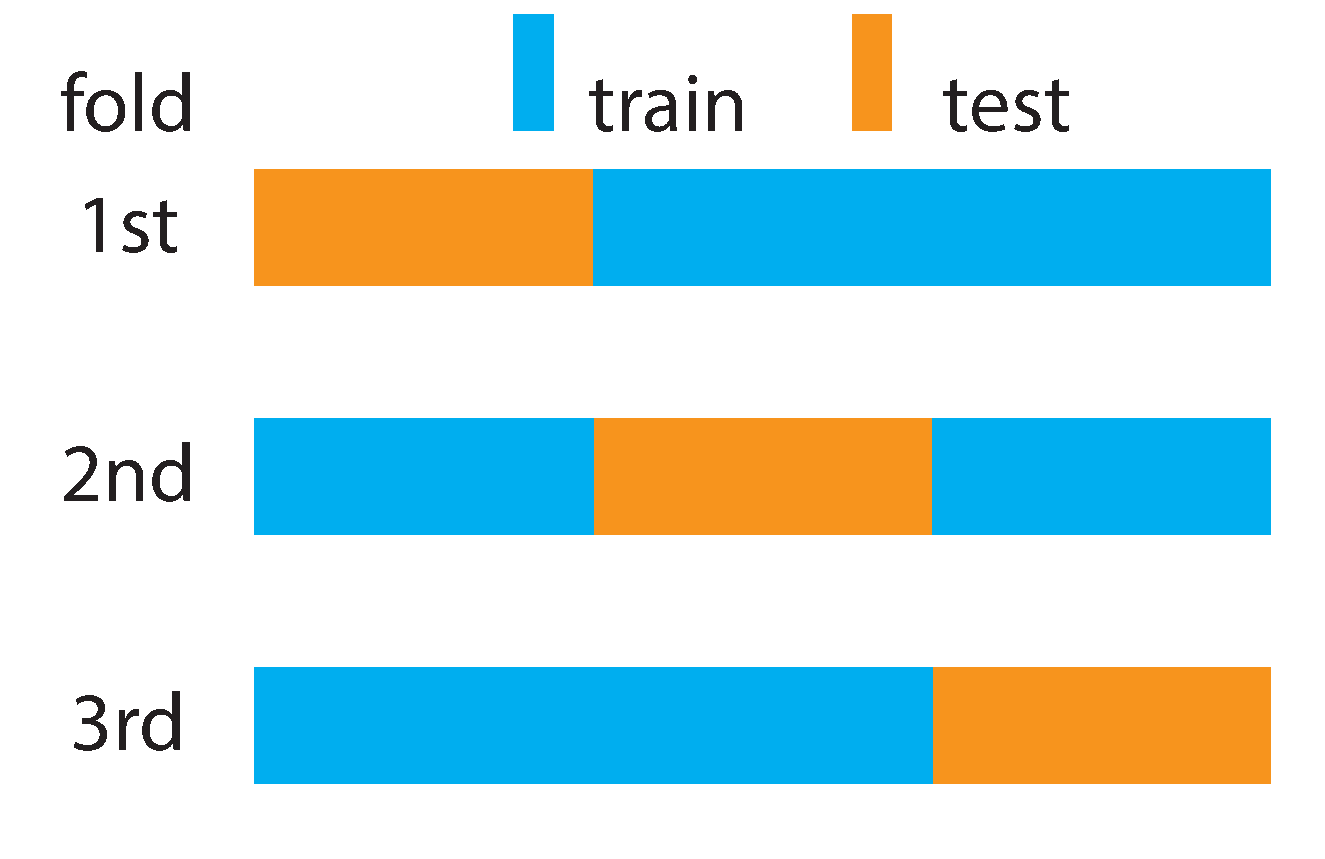
\includegraphics[width=0.8\textwidth]{figures/lec7_testSet_kFolds.pdf}}
	\end{figure}
	
	\onslide<2->
	$\implies$ average log-likelihood across all posterior $\theta$ across all folds. \textbf{Note:} no need for overfitting correction!
	
\end{frame}

\begin{frame}
	\frametitle{Cross validation: issues for consideration}
	
	\begin{itemize}
		\item<2-> Cross-validation method should reflect eventual use of model. For example, if predicting individual data points is most important use leave-one-out.
		\item<3-> Manual-refitting the model for each train/set can be costly $\implies$ k-folds is less time-consuming than leave-one-out.
		\item<4-> Leave-one-out may be difficult for hierarchical models where data is naturally grouped $\implies$ use k-folds where one fold = one group.
		\item<5-> Remember cross-validation is still an approximation to out-of-sample estimation $\implies$ best to get new and independent data set!
	\end{itemize}
	
\end{frame}

\begin{frame}
	\frametitle{Bayes factors}
	\onslide<2-> An alternative approach is to use Bayes factors to choose between models:
	
	\onslide<3->
	\begin{equation}
	\frac{p(\text{model 1}|X)}{p(\text{model 2}|X)} = \textcolor{blue}{\frac{p(X|\text{model 1})}{p(X|\text{model 2})}}\times \frac{p(\text{model 1})}{p(\text{model 2})}
	\end{equation}
	
	where \textcolor{blue}{blue} expression is known as the \textbf{Bayes factor.}
	
	\onslide<4->
	$\implies$ requires:
	\begin{itemize}
		\item<5-> \textit{a priori} specification of our preferences over models (not simple for models with different dimensions.)
		\item<6-> Calculate $p(X|\text{model})$ -- known as the \textbf{marginal likelihood} for a model. \onslide<7-> Calculate by,
		\begin{equation}
		p(X|\text{model}) = \int \underbrace{p(X|\theta,\text{model})}_{\text{likelihood}} \times \underbrace{p(\theta|\text{model})}_{\text{prior}}\;\mathrm{d}\theta
		\end{equation}
	\end{itemize}
	
\end{frame}

\begin{frame}
	\frametitle{Problem with Bayes factors 1: marginal likelihood's sensitivity to priors}
	\onslide<2-> Suppose $X\sim \text{binomial}(10,\theta)$ likelihood, and $\theta\sim \text{beta}(a,a)$ prior. \onslide<3-> \textbf{Question:} how does the marginal likelihood vary as $a\uparrow$?
	
	\onslide<4->
	\begin{figure}[t]
		\centerline{\animategraphics[width=0.85\textwidth,controls,buttonsize=1em,buttonfg=0.5]{2}{animations/lec7_marginalLikelihood}{1}{20}}
	\end{figure}
	
\end{frame}

\begin{frame}
	\frametitle{Problem with Bayes factors 2: difficulty estimating marginal likelihood}
	\onslide<2-> For most problems $\theta={\theta_1,...,\theta_p}$,\onslide<3->
	\begin{align}
	p(X|\text{model}) = \int...\int &p(X|\theta_1,...,\theta_p,\text{model}) \times\\
	& p(\theta_1,...,\theta_p|\text{model})\;\mathrm{d}\theta_1 ...\mathrm{d}\theta_p
	\end{align}
	
	\onslide<4-> $\implies$ integral too difficult to compute in practice. \onslide<5-> But can approximate using Monte Carlo integration,
	
	\begin{equation}
	p(X|\text{model}) \approx \frac{1}{S}\sum_{s=1}^{S} p(X|\theta_{1s},...,\theta_{ps},\text{model})
	\end{equation}
	
	where $\theta_{1s},...,\theta_{ps}\sim p(\theta_1,...,\theta_p|\text{model})$, i.e. priors.

	
\end{frame}

\begin{frame}
	\frametitle{Problem with Bayes factors 2: difficulty estimating marginal likelihood}
	\begin{equation}
	p(X|\text{model})\approx \frac{1}{S}\sum_{s=1}^{S} p(X|\theta_{1s},...,\theta_{ps},\text{model})
	\end{equation}
	
		\onslide<2-> However simple Monte Carlo integration is very slow to converge, particularly when there is a mismatch between the position of the prior and likelihood. \onslide<3-> Solutions exist, for example:
		
		\begin{itemize}
			\item<4-> Bayesian Monte Carlo.
			\item<5-> Importance Sampling Annealing.
			\item<6-> Adiabatic Monte Carlo.
		\end{itemize}
		
		\onslide<7->
		But still early days in the research.
\end{frame}

\begin{frame}
	\frametitle{Bayes factors: summary}
	\begin{itemize}
		\item<2-> Require us to specify priors over model choice and calculate marginal likelihood.
		\item<3-> Marginal likelihood is highly sensitive to priors, even for nuisance parameters.
		\item<4-> Marginal likelihood hard to calculate exactly (multi-dimensional integral), and so approximate using sampling.
		\item<5-> $\implies$ simple Monte Carlo is slow to converge.
	\end{itemize}
\end{frame}


\begin{frame}
	\frametitle{Model selection: summary}
	
	\begin{itemize}
		\item<2-> Model selection inevitable part of scientific process $\implies$ need a method for choosing between rival models.
		\item<3-> Posterior predictive checks useful in model building process but use predictive performance to select between hypotheses.
		\item<4-> Out-of-sample predictive performance is our aim.
		\item<5-> Two methods:
		\begin{itemize}
			\item[-]<6-> Post-hoc correction: Approximate LOO-CV using ``loo'' R package, or failing that use WAIC.
			\item[-]<7-> (Better) cross-validation: leave-one-out or k-folds.
		\end{itemize}
		\item<8-> Bayes factors can be useful for model selection although need to be careful!
	\end{itemize}
	
\end{frame}


\begin{frame}
	\frametitle{Modelling tips}
	\begin{itemize}
		\item<2-> Aim to graph data in the most enlightening way for eventual model use; this is difficult and requires going through a lot of useless visualisations. Try \textit{grammar of graphics} approaches like \textit{ggplot}.
		\item<3-> Start simple with modelling and build up complexity as needed.
		\item<4-> Use creative posterior predictive checks to test model assumptions.
		\item<5-> Read books on inference $\implies$ build up knowledge of models/frameworks.
		\item<6-> Present your work to colleagues; the process of preparing for presentation as well as the feedback itself is always useful.
		\item<7-> When in doubt use hierarchical models.
	\end{itemize}
	
\end{frame}


\end{document}

